
\hypertarget{remote}{} 
\section{Remote access}

Since one of the main target groups for LessLinux are network admins, easy remote access to running LessLinux instances was one of the goals during development. Currently access via \index{SSH} SSH and \index{VNC} VNC is supported, both together result in encrypted VNC. Reverse VNC allows for easy remote support on machines that are behind NAT routers and firewalls. RDP access is work in progress. 

\hypertarget{ssh}{} 
\subsection{SSH}

LessLinux is usually shipped with the OpenSSH secure shell server. However this is disabled in most builds by adding it to the \texttt{skipservices=|servic1|service2|} boot command line. To start the OpenSSH server, remove \texttt{ssh} from \texttt{skipservices}.

\Warning{
Placing the hash for the root password in the boot command line, transferring it over a hostile network or netbooting with SSH machine keys (or root's private SSH keys) make eavesdropping easy. Use those options just in networks that are considered safe. Also consider locking down the local consoles when LessLinux is netbooted in order to do adminstrative tasks via SSH to prevent local users from manipulating the machine.
}

\subsubsection{Login with password}

To login with password use the possibility to add files to the initramfs by adding \texttt{/etc/lesslinux/root.hash} that contains the MD5 hash of the root password. You can generate this hash with the command

\begin{verbatim}
openssh passwd -1 
\end{verbatim}

You might also specify the base64 encoded MD5 hash of the root password via boot command line. Since the \texttt{=} character which is used for indicating padding in base64 is not valid, you will have to pad the hash with one or more spaces (usually one) until the base64 string does not end on \texttt{=}. Those spaces are removed after decoding:

\begin{verbatim}
hash=` openssl passwd -1 `
echo "$hash " | base64 
\end{verbatim}

The result must look like:

\begin{verbatim}
JDEkTktlL3NSRHIkd1owLzJ5UjJDTVdlMnZPY0NaSGRuMSAK
\end{verbatim}

The resulting parameter for the boot command line:

\begin{verbatim}
roothash=JDEkTktlL3NSRHIkd1owLzJ5UjJDTVdlMnZPY0NaSGRuMSAK
\end{verbatim} 

\subsubsection{Public key login}

Use the possibility to add files to the initramfs by preparing a CPIO archive that contains all the host keys placed in \texttt{/etc/openssh} as well as the needed \texttt{/root/.ssh/authorized\_keys}. Make sure permissions fit and add this CPIO archive as the last file to the bootloader or concatenate it to the initramfs if you use a bootloader that allows just one initramfs. If permissions are correct and the OpenSSH daemon is started you can connect with public key login afterwards.

\subsection{VNC}

Virtual Network Computing or \emph{VNC} is a simple, easy to implement protocol used to gain access to remote computers. It is the basis for Apple's remote administration tool. Clients are available for nearly every operating system as well as for smartphones and as Java applet. In LessLinux VNC can be used to mirror a local X server - which can be either a graphical console or an invisible virtual frame buffer.

\Warning{The VNC protocol does not use encryption! This means all keyboard input and all screen output can easily be eavesdropped. Combine VNC with an SSH tunnel if you need some minimum security.}

\subsubsection{VNC for incoming connections}

The easiest way to access a running LessLinux system is mirroring the local Xserver. Specify

\begin{verbatim}
x11vnc=|remote|
\end{verbatim}

to enable VNC access without password. You might specify a clear text password as second argument:

\begin{verbatim}
x11vnc=|remote|password|
\end{verbatim}

VNC uses port 5900 as default. The current IP address is usually shown on the first console (\texttt{Ctrl+Alt+F1}). 

\subsubsection{Reverse VNC}

If a host that booted LessLinux is running behind a firewall or NAT router, incoming connections might not be possible. With reverse VNC the LessLinux host tries to establish an outgoing connection to the IP address or hostname specified as target (on port 5500):

\begin{verbatim}
x11vnc=|reverse|target|
\end{verbatim}

On a Linux target machine you usually run 

\begin{verbatim}
vncviewer -listen
\end{verbatim}

or use the graphical application Remmina to work with reverse VNC connections.

\subsubsection{Headless access}
 
Specify \texttt{x11vnc=...} as mentioned above to enable VNC access. To run headless access instead of the local X server you have to disable it and replace it by Xvfb - the virtual frame buffer X server, which is done with the additional parameter 

\begin{verbatim}
xvfb=1280x800x32
\end{verbatim}
 
The \texttt{1280x800x32} tells Xvfb to start with an 1280x800 resolution and 32 bit color depth. All values that make sense (they should resemble real world resolutions) are allowed.

\subsubsection{Tunnel VNC over SSH}

The security implecations of VNC are described earlier in this chapter. If you want to use VNC in hostile environments, enable  \hyperlink{ssh}{SSH access}. Then bind the listening port for VNC to localhost only by specifying:

\begin{verbatim}
x11vnc=|local|
\end{verbatim}

On the machine that is used to access the LessLinux with running VNC you then have to run SSH with port forwarding, on unix like operating systems:

\begin{verbatim}
ssh -L 5900:localhost:5900 lesslinux-host
\end{verbatim}

On the machine connecting via SSH, VNC's port 5900 is now available at \texttt{localhost}, point your VNC viewer to \texttt{localhost} or \texttt{127.0.0.1}. Depending on the viewer it may be necessary to specify the priority of encodings (if you are using \texttt{vncviewer} from TightVNC, see the man page regarding \texttt{-encodings}.

\subsection{RDP}

Remote access via Microsofts Remote Desktop Protocol \index{RDP} based on \texttt{xrdp} is in experimental state. Specify 

\begin{verbatim}
xrdp=1
\end{verbatim}

to enable the VNC-to-RDP gateway. This requires a running VNC server, at least listening on the local loopback interface. Of course you can enable RDP with an VNC server that mirrors the local display or headless. We suggest using

\begin{verbatim}
x11vnc=|local|secret| xvfb=1280x800x16 xrdp=1
\end{verbatim}

to enable a headless VNC server that listens on 127.0.0.1, color depth fset to 16 bit. The password ,,secret'' will then be prompted upon RDP login. All traffic is encrypted which minimizes the risk of sniffing.

\begin{figure}[htbp]
\center{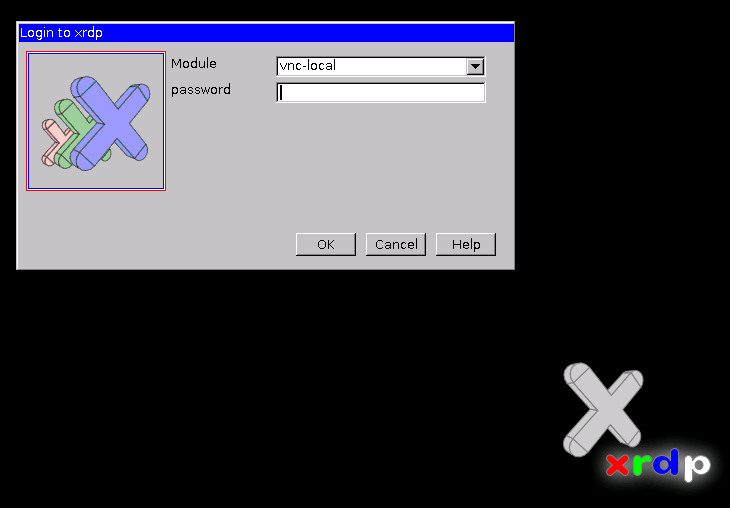
\includegraphics[width=8cm]{admin/xrdp.png}}
\caption{\label{fig:xrdp} Xrdp provides a simple VNC-to-RDP gateway, this comes handy if you want to access a machine running LessLinux from a Windows machine.}
\end{figure}

\subsection{Xpra}

,,X persistent remote applications'' is a relatively unknown, yet very efficient way of saemlessly exporting X11 applications to another computer. See \href{https://www.xpra.org}{www.xpra.org} for details.  The connection between machines is usually done with a SSH tunnel. If the connection is lost, all applications and usually even their positions are restored upon re-connect. Xpra needs a running SSH server, so make sure to enable it and set a password or provide a key before enabling Xpra. Enable Xpra with

\begin{verbatim}
xpra=1
\end{verbatim}

Then connect on another computer with Xpra installed with the command:

\begin{verbatim}
xpra attach ssh:root@12.34.56.78:100 
\end{verbatim}

After providing the password you will get a single terminal window from which you can start any X11 application. To change the default app that is started, provide the full path when enabling Xpra:

\begin{verbatim}
xpra=/path/to/program
\end{verbatim}




